\subsection{Frontend}

\begin{frame}{Frontend}

	\begin{figure}
	  \begin{center}
	    \leavevmode
	      \includegraphics[width = .75\textwidth]{frontend}
	    \caption{Team Frontend}
	  \end{center}
	\end{figure}

\end{frame}

\begin{frame}{Frontend}

	\pause
	\"Ubersicht:
	\pause
	\begin{itemize}
		\item Softwaretechnik
		\pause
		\item Technische Aspekte
	\end{itemize}

\end{frame}

\pagepreak


\begin{frame}{Frontend: Softwaretechnik}
	
	\pause
	\begin{itemize}
		\item Sechs Teammitglieder
		\pause
		\item Austausch mit Haskell-Gruppe: Design der AST-Datei
		\pause
		\item Kommunikation wie im Organisationsteil erw\"ahnt
		\pause
		\item T\"atigkeitsfelder:
		\pause
		\begin{itemize}
			\item Lexer
			\pause
			\item Parser
			\pause
			\item AST Serialisierung/Deserialisierung
			\pause
			\item Rail-Testcases
			\pause
			\item Testing-Framework
		\end{itemize}
	\end{itemize}
	
\end{frame}

\pagebreak
\begin{frame}{Frontend: Softwaretechnik}

	\begin{itemize}
		\item Wichtige Erkenntnisse
		\pause
		\begin{itemize}
			\item Gelernte Theorie l\"asst sich nur begrenzt anwenden
			\pause
			\item Praktische Umst\"ande verlangen individuelle L\"osungen
			\pause
			\item Ein guter Entwurf spart enormen Aufwand
		\end{itemize}
	\end{itemize}
	
\pagebreak

\end{frame}

\begin{frame}{Frontend: Softwaretechnik}

\begin{figure}
  \begin{center}
    \leavevmode
      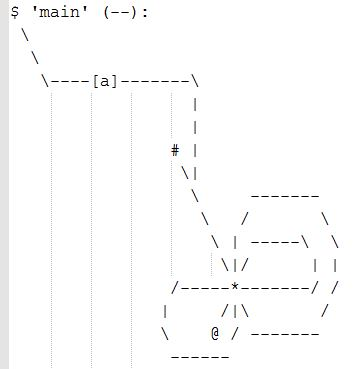
\includegraphics[width = .5\textwidth]{rail}
    \caption{Grammatik hierf\"ur?}
  \end{center}
\end{figure}

	
\end{frame}

\begin{frame}{Frontend: Technisches}

\begin{figure}
  \begin{center}
    \leavevmode
      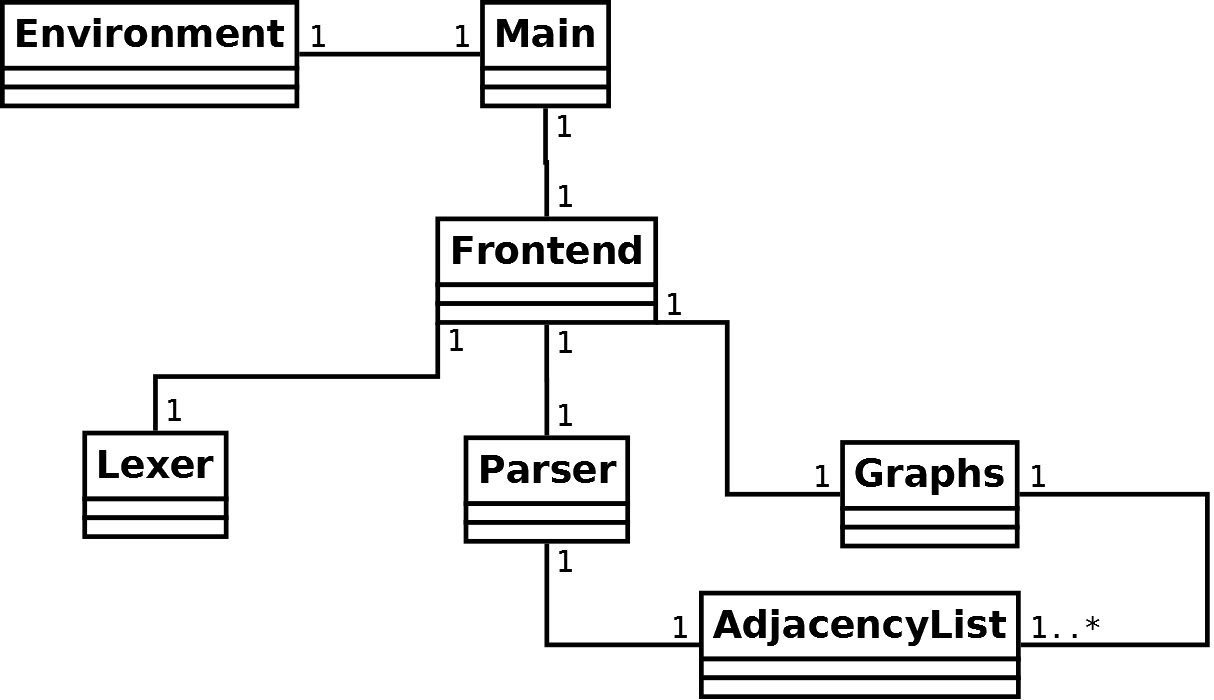
\includegraphics[width = \textwidth]{frontenduml}
    \caption{Klassendiagramm Frontend}
  \end{center}
\end{figure}

\end{frame}

\begin{frame}{Frontend: Technisches}

Die Hauptarbeit geschieht im Parser:
\pause
\begin{itemize}
	\item Durchlaufen der Funktion anhand der Schienen
	\pause
	\item Aufbau einer Graph-Struktur durch den Parser
	\pause
	\item F\"ur jeden gesehenen Rail-Befehl wird gespeichert:
	\pause
	\begin{itemize}
		\item Position
		\pause
		\item Richtung
		\pause
		\item Befehl
		\pause
	\end{itemize}
	\item Verkn\"upfen dieser Informationen mit dem Knoten verhindert mehrfaches Parsen
	\pause
	\item Verzweigungen durch rekursive Selbstaufrufe
	\pause
	\item F\"ur anonyme Funktionen (Lambda) werden neue Funktionsnamen generiert und die Funktionen geparst
	\pause
	\item Erzeugt f\"ur jede Rail-Funktion einen Graphen
\end{itemize}

\end{frame}
